\documentclass[]{article}

\usepackage{tikz}
\usepackage{pgfplots}
\usepackage{listings}
\usepackage{geometry}
\usepackage{babel}
\usepackage{subcaption}

%opening
\title{Concurrent Game of Life}
\author{
	Kai Hulme\\
	Computer Science\\
	\texttt{kh16747@my.bristol.ac.uk}
	\and
	Jack Bond-Preston\\
	Computer Science\\
	\texttt{jb17662@my.bristol.ac.uk}
}
\date{December 2018}
\lstset{
	language=C,
	basicstyle=\small,
	stringstyle=\ttfamily
}
\geometry{margin=0.9cm}
\pagenumbering{gobble}

\begin{document}

\maketitle
\clearpage

\section{Functionality and Design}
Our implementation of Game of Life uses a distributor and a set of workers. Each round of the game, the distributor gives each worker the section of the board it is responsible for processing and at the end of the round, the workers all send back this section and it is combined by the distributor back into the one complete board.\\

The distributor and workers all run in parallel, along with threads for receiving button input, handling timing, and processing orientation data. The channels between all threads are standard synchronised channels.\\

We decided to unparallelise some of the functions to free up resources - reading and writing to files as well as setting LED output states. These were originally threads with loops receiving inputs from channels, but we decided they did not need to be always running, and it was ok for them to block the distributor thread while running, as nothing else needed to be done in parallel as they were processing.\\

Originally, all cells were read in and stored as \lstinline{uchar}s. This uses 8 bits per cell, even though a cell can only have 2 states - dead or alive. This meant it was possible to use bit packing to reduce cells to a single bit and make better use of the board's limited memory. When the image is generated or loaded from a file, all the cells are packed into a \lstinline{b_int}. Each bit of this integer is then set to a corresponding cell. When the worker is processing the cells, it unpacks each bit as it uses it - the board is only ever stored in memory in the packed form. This results in the program being able to handle much larger board sizes.\\

The number of workers can be changed and the distributor will then split the board into horizontal strips, dividing it evenly between the given number of workers. Two extra rows of cell data are prepended and appended to this section, as the row above and below are needed to find the state of the cells in the next turn. These strips are then distributed to the respective workers. The workers then compute the next turn state of all the cells and send these back to the distributor. This method of distribution is a simple star topology, with the distributor being at the centre.\\

Each turn, the worker iterates through each of it's given cells and uses a function to apply the game of life rules and find whether this cell will be dead or alive next turn. To this function we have applied several optimisations:
\begin{itemize}
	\item The function can stop early if it reaches a state where checking more neighbours will not affect the outcome of the cell's state. For example, if the cell was alive and four neighbour cells were found to be alive, the function returns a dead cell early - as no future neighbours can affect this outcome.
	\item If a packed int of cells is found to be 0 (all its cells are dead), the one above is found to be 0, and a number of ints below are found to be 0, the worker can then skip processing this vertical block of cells, and only process the left- and right-most cells of these strips as all the other contained cells can be assumed to be dead.
\end{itemize}

We found the optimal way to distribute work across the board was to have all the workers on tile 1, and the distributor and all other minor I/O and timing threads on tile 0. This was the best way to equally distribute memory usage between the two tiles - the distributor holds the entire board in memory, and when the workers are processing, they together hold the whole board in memory, resulting in approximately equal memory usage between tiles. Normal, synchronous \lstinline{chan}s were used for communication between threads - however if the worker count is set to 4 or less the channels between the workers and distributor are set to asynchronous \lstinline|streaming chan|s. These are faster as the distributor does not need to wait for handshaking when sending the board data - however the XMOS board is limited to 4 streaming channels across the tiles, so we could not streaming channels with 8 workers, leaving a trade-off between worker count and channel speed.\\

Some of the constant values in the program will dynamically affect how the board is processed:
\begin{itemize}
	\item If the board size is 16x16 the bits are packed into 16-bit \lstinline|uint16_t|s. Otherwise, 32-bit \lstinline|uint32_t|s are used.
	\item If the worker count is 4 or less, the channel type is set to \lstinline|streaming chan|, otherwise it is just \lstinline|chan|.
\end{itemize}

\clearpage

\section {Tests and Experiments}

\subsection{Image Outputs}
Here are the output images from the provided input images at various round numbers.

\begin{figure}[!htb]
\begin{subfigure}{0.16\textwidth}
	\centering
	
\includegraphics[width=\linewidth]{images/16x16_2_Rounds.png}
	\caption{16x16 - 2}
\end{subfigure}
\begin{subfigure}{0.16\textwidth}
	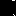
\includegraphics[width=\linewidth]{images/16x16_100_Rounds.png}
	\caption{16x16 - 100}
\end{subfigure}
\begin{subfigure}{0.16\textwidth}
	\centering
	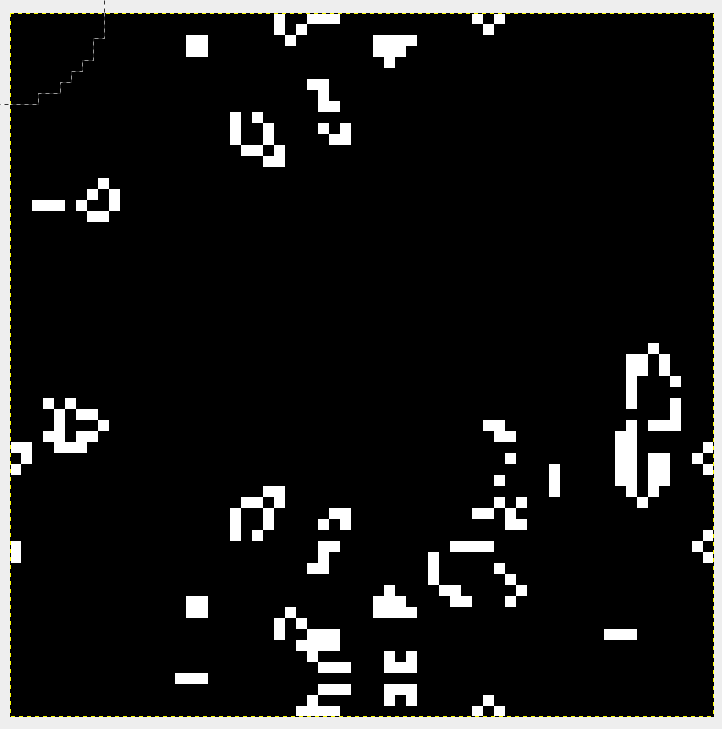
\includegraphics[width=\linewidth]{images/64x64_100_Rounds.png}
	\caption{64x64 - 100}
\end{subfigure}
\begin{subfigure}{0.16\textwidth}
	\centering
	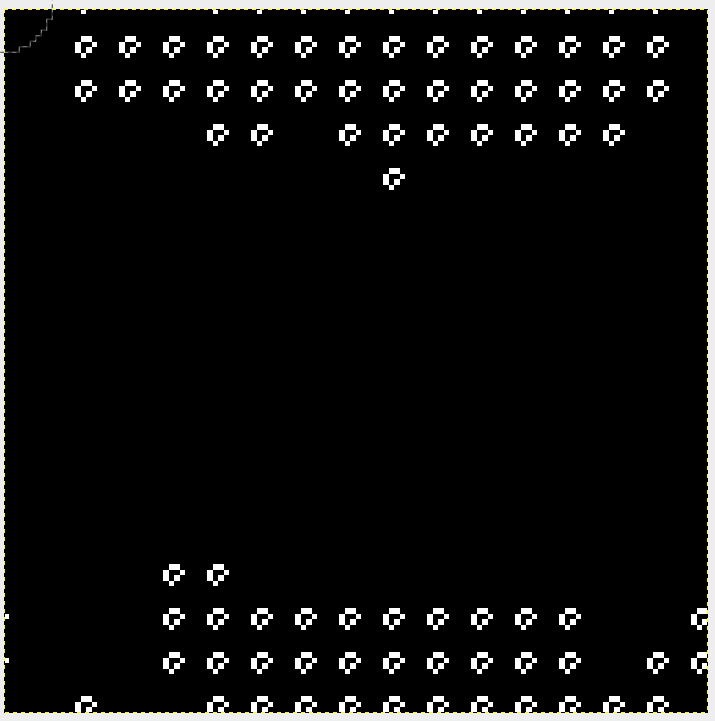
\includegraphics[width=\linewidth]{images/128x128_100_Rounds.png}
	\caption{128x128 - 100}
\end{subfigure}
\begin{subfigure}{0.16\textwidth}
	\centering
	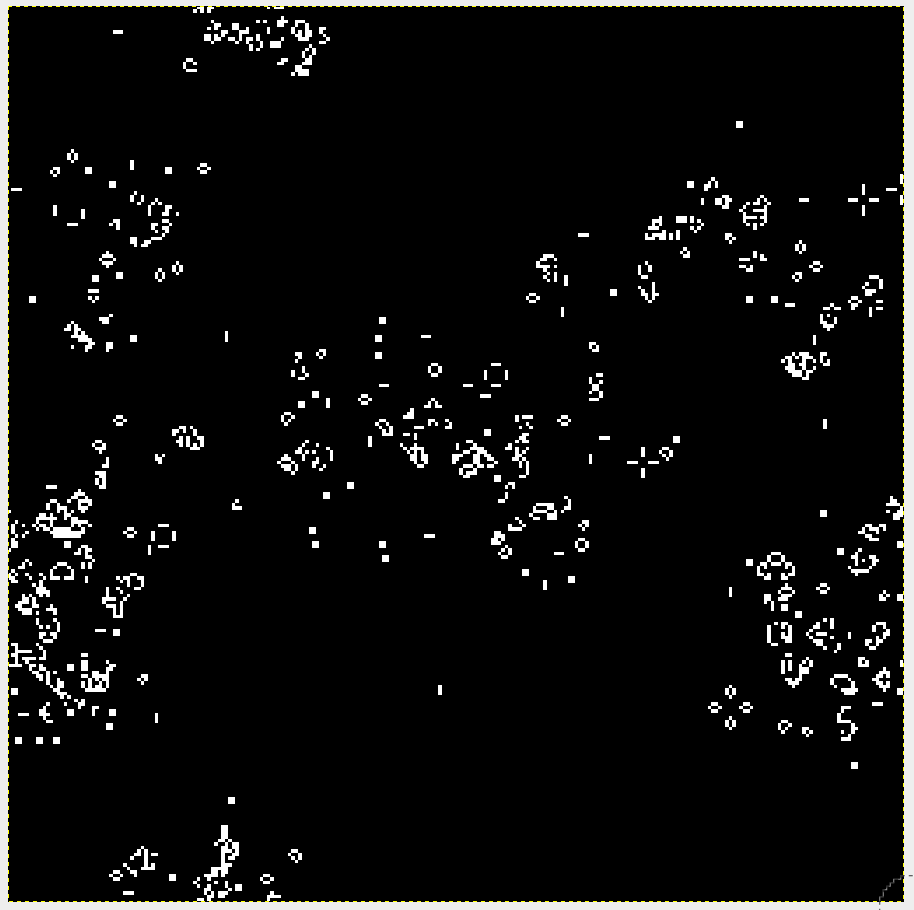
\includegraphics[width=\linewidth]{images/256x256_100_Rounds.png}
	\caption{256x256 - 100}
\end{subfigure}
\begin{subfigure}{0.16\textwidth}
	\centering
	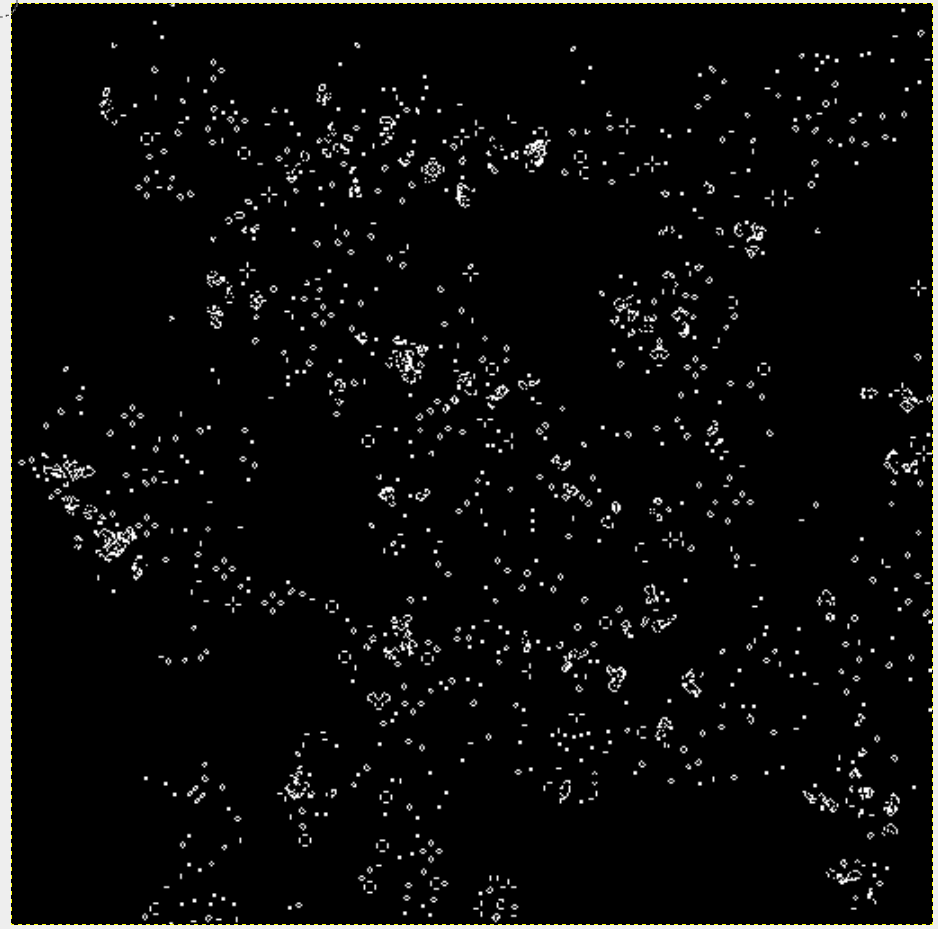
\includegraphics[width=\linewidth]{images/512x512_100_Rounds.png}
	\caption{512x512 - 100}
\end{subfigure}
\caption{Image Outputs (Size - Rounds)}
\end{figure}

\subsection{Memory Usage}
Before the implementation of bit packing, the board was not able to load or process the 512x512 example image. The memory constraint check failed on tile 0, with \texttt{451588 / 262144} of its memory being expended. This was the entire board stored unpacked, as well as some other sections of the board stored on workers, some of which were also running on tile 0 at the time.\\
After the implementation of bit packing, boards of up to size 1312 x 1312 were able to be loaded and processed. This was the absolute maximum, increasing the size to 1344 resulted in a memory constraint failure with \texttt{262144 / 262144} of memory being used on tile 0.\\
There was no good solution for further improving the board size capacity, due to the implementation having to store the entire board on the distributor which lives on one tile. The board's limited per-tile memory meant it was impossible to load a larger board onto this tile, and to potentially further increase the size the distributor would have to be split across tiles as well which was not practical.

\subsection{Processing Speed}
We progressively made improvements to the algorithm to optimise the runtime to get it as fast as possible. After implementing bit packing to reduce memory usage, we found that packing and unpacking did not slow the program down - in fact it was slightly faster, likely due to there being much less data to send through channels. We did some experimentation with worker counts and found that upping the worker count from 4 to 8 resulted in a 25\% improvement in round time (on the original, non-optimised algorithm.) After this we kept using 8 workers and bit packing, and built upon this, making several improvements that focussed on runtime rather than memory usage:

\begin{figure}[!htb]
\begin{subfigure}{0.63\textwidth}
\centering
\begin{tikzpicture}[scale=0.8]
\begin{axis}[
xtick=data,
ylabel={Speed ($ = \frac{100}{time}$) Increase from Original Algorithm (\%)},
xlabel={Board Length/Width - Square (\# cells)},
legend style={
	at={(0.5, -0.15)},
	anchor=north,
	legend columns=2,
	/tikz/every even column/.append style={column sep=0.5cm}
},
ybar,
symbolic x coords={16, 64, 128, 256, 512, 1024, 1312},
bar width=6.5,
width=12cm,
ymajorgrids,
legend cell align=left
]

\addplot
coordinates {
	(16, 15)
	(64, 13)
	(128, 13)
	(256, 15)
	(512, 8)
	(1024, 8)
	(1312, 5)
};

\addplot
coordinates {
	(16, 66)
	(64, 66)
	(128, 112)
	(256, 85)
	(512, 88)
	(1024, 10)
	(1312, 15)
};

\addplot
coordinates {
	(16, -3)
	(64, -9)
	(128, 12)
	(256, 4)
	(512, 12)
	(1024, -16)
	(1312, -12)
};

\addplot
coordinates {
	(16, 2)
	(64, -8)
	(128, 19)
	(256, 39)
	(512, 50)
	(1024, -14)
	(1312, -10)
};

\legend{
	8 Worker Less Checks,
	8 Worker Fully Optimised,
	4 Worker Normal Channels,
	4 Worker Streaming Channels
}
\end{axis}
\end{tikzpicture}
\caption{Optimisation effects on speed}
\label{fig:optimisations}
\end{subfigure}
\begin{subfigure}{0.33\textwidth}
\centering
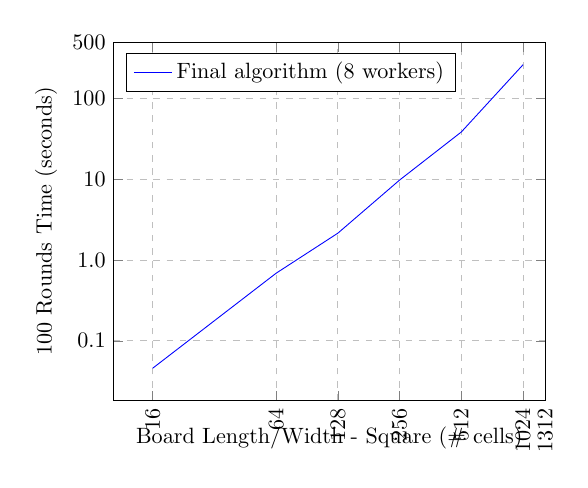
\begin{tikzpicture}[scale=0.8]
\begin{axis}[
xlabel={Board Length/Width - Square (\# cells)},
ylabel={100 Rounds Time (seconds)},
xmin=0, xmax=1312,
ymin=0, ymax=500,
xtick={16, 64, 128, 256, 512, 1024, 1312},
xticklabels={16, 64, 128, 256, 512, 1024, 1312},
x tick label style={rotate=90, anchor=east},
ytick={0.1, 1.0, 10, 100, 500},
yticklabels={0.1, 1.0, 10, 100, 500},
legend pos=north west,
grid style=dashed,
ymode=log,
xmode=log,
log basis x=2,
grid=both,
xlabel style={
	at={(0.5, -0.05)}
}
]

% 8 workers skipping dead areas
\addplot[
color=blue
]
coordinates {
	(16, 0.045632)
	(64, 0.686599)
	(128, 2.15193)
	(256, 9.795099)
	(512, 38.607723)
	(1024, 263.114624)
};

\legend{
	Final algorithm (8 workers)
}

\end{axis}
\end{tikzpicture}
\caption{Relationship between board size and round time}
\label{fig:finalgraph}
\end{subfigure}
\caption{Performance graphs}
\end{figure}

\begin{itemize}
	\item Less neighbour checks - the function that finds the next state for a cell based upon it's neighbour originally always checked all 8 neighbours of the cell before returning the next state. We realised this was not necessary, there are many cases where you can return early as the remaining cells cannot change the output of the function.
	\begin{lstlisting}[basicstyle=\scriptsize, numbers=left]
if (currentValue == ALIVE) {
	if (liveNeighbours > 3) return DEAD;
	else if (neighboursChecked == 7) {
		if (liveNeighbours == 0) return DEAD;
		if (liveNeighbours == 2) return ALIVE;
	} else if (neighboursChecked == 8) {
		if (liveNeighbours > 1 && liveNeighbours < 4) return ALIVE;
		return DEAD;
	}
} else {
	if (neighboursChecked - liveNeighbours == 6) return DEAD;
	else if (neighboursChecked == 8) {
		if (liveNeighbours == 3) return ALIVE;
		return DEAD;
	}
}
	\end{lstlisting}
	As you can see in the blue bar in Figure \ref{fig:optimisations}, this optimisation made a reasonably large, and fairly constant improvement on speed (an average of 12\% compared to the original algorithm)
	
	\item We found a lot of the given images either contained large dead areas, or developed them after time. These areas were a waste of computation as they would always stay dead after processing. In the worker function, we implemented a way to skip vertical strips of dead cells. Each time a packed int of cells is being checked, the worker checks if the int's value is 0 (which means all the cells within it are dead.) If this is the case, it checks if the int above it is completely dead, and if one or more below are completely dead. For this area of dead cells, only the outermost border cells are computed on. The impact of this optimisation varies based upon the input image, as shown in the red bar in Figure \ref{fig:optimisations} (this also includes the reduced neighbour checks optimisation.) For the provided input images, which often featured a reasonably large amount of dead cells, it resulted in a large speed-up (an average of 83\% faster than the original algorithm.) For the on-board randomly generated images, it did not have a particularly large effect as they tended to not have or develop many large dead areas. We also tested using 16-bit rather than 32-bit packed integers - the trade-off being it would be able to skip more often, but would result in more checks. We found the difference was negligible and stuck with 32-bit (except for board sizes below 32). 
	
	\item We also experimented with the use of asynchronous channels instead of the regular channels we had been using. We switched the channels between the distributor and workers to streaming channels. We reasoned this would result in a speed increase due to less overhead on sending data through channels, as asynchronous channels do not use handshaking. This allows the distributor to send off the board data much faster without waiting for a response from the workers. However, we discovered that the XMOS xCORE 200 eXplorer board does not have the capacity for 8 streaming channels across the two tiles, so we could only use streaming channels with 4 workers. We experimented with runtime with 4 workers with and without streaming channels (with all previous optimisations already implemented) and found that whilst streaming channels do increase speed, the increase is not enough to be faster than 8 workers without them (see brown and grey bars in Figure \ref{fig:optimisations}).
\end{itemize}
In the end, we added the less neighbour checks optimisation and the dead area skipping. We did not use streaming channels unless the worker count has been set to 4 or less, as 8 workers with non-streaming channels is still much faster. As you can see in Figure \ref{fig:finalgraph}, the logarithm of the 100 rounds run time scales linearly with the log of the board length.


\subsection{Limitations}
The main limitations we encountered were:
\begin{itemize}
	\item Lack of memory on the board - this meant we could only load or generate images of a certain size before one or both of the tiles had their memory exhausted.
	\item Streaming channel limit - we were unable to create 8 streaming channels due to hardware limitations, which could have sped up the program by a reasonable margin.
	\item Lack of cores - we were limited in our number of workers by the number of cores on the board.
	\item Slow read/write times of .pgm files - we could not properly test our skipping algorithm on larger images as 1024x1024 images would take upwards of 15 minutes to load. These randomly generated images are very random, thus they do not have a lot of dead space (like some of the provided images) and the dead space skipping optimisation had little effect on them.
\end{itemize}
\clearpage

\section {Critical Analysis}

\subsection{Results}
The maximum size image our program can process is 1312 x 1312 - these images are randomly generated on the board due to extremely long load times.\\

Here are the final version's runtimes for various sized boards:\\

\begin{tabular}{|c|c|c|}
	\hline 
	Board  Width (Square) & 100 Rounds Time ($seconds$) & Speed ($rounds$ $second^{-1}$) \\ 
	\hline 
	16 & 0.045632 & 2191.4446 \\ 
	\hline 
	64 & 0.686599 & 145.6454204 \\ 
	\hline 
	128 & 2.151930 & 46.46991305 \\ 
	\hline 
	256 & 9.795099 & 10.20918727 \\ 
	\hline 
	512 & 38.607723 & 2.590155343 \\ 
	\hline 
	1024 (generated) & 263.114624 & 0.380062493 \\ 
	\hline 
	1312 (generated) & 436.016052 & 0.229349354 \\ 
	\hline              
\end{tabular}

\subsection{Improvements}
The memory efficiency of the program could not easily be improved. The distributor has to hold the entire board, and the board is already packed around its minimum possible size. The only way to increase the maximum board size would be to make the workers process 3 rows at once and split the board across 2 distributors on different tiles, so that the memory could be used better.

The runtime of the program could be further improved. For example, the distributor could just send the size of the gaps between alive cells and the worker could fill its board from this information - resulting in much less data being sent if the board contains many dead cells.

In general, skipping dead areas seemed like the main optimisation that could be made. We feel our implementation is okay, but then are definitely more optimal ways to do it - albeit likely more complex. We found it was often a trade-off between making more checks to be able to skip more areas - it only pays off if the skipped areas time saved outweighs the additional checks.

\subsection{Conclusion}
We have made a memory efficient algorithm - each cell takes the minimum possible amount of memory and a board with over 1.7million cells can be loaded and processed.\\
We made several optimisations over the process which resulted in an overall very large increase in performance, in some cases over 100%.

\end{document}
